\thispagestyle{timhieukhoahocnone}
\pagestyle{timhieukhoahoc}
\everymath{\color{timhieukhoahoc}}
\blfootnote{$^1$\textcolor{timhieukhoahoc}{Viện Sinh thái và Môi trường Đông Dương.}}
\graphicspath{{../timhieukhoahoc/pic/}}
\begingroup
\AddToShipoutPicture*{\put(0,616){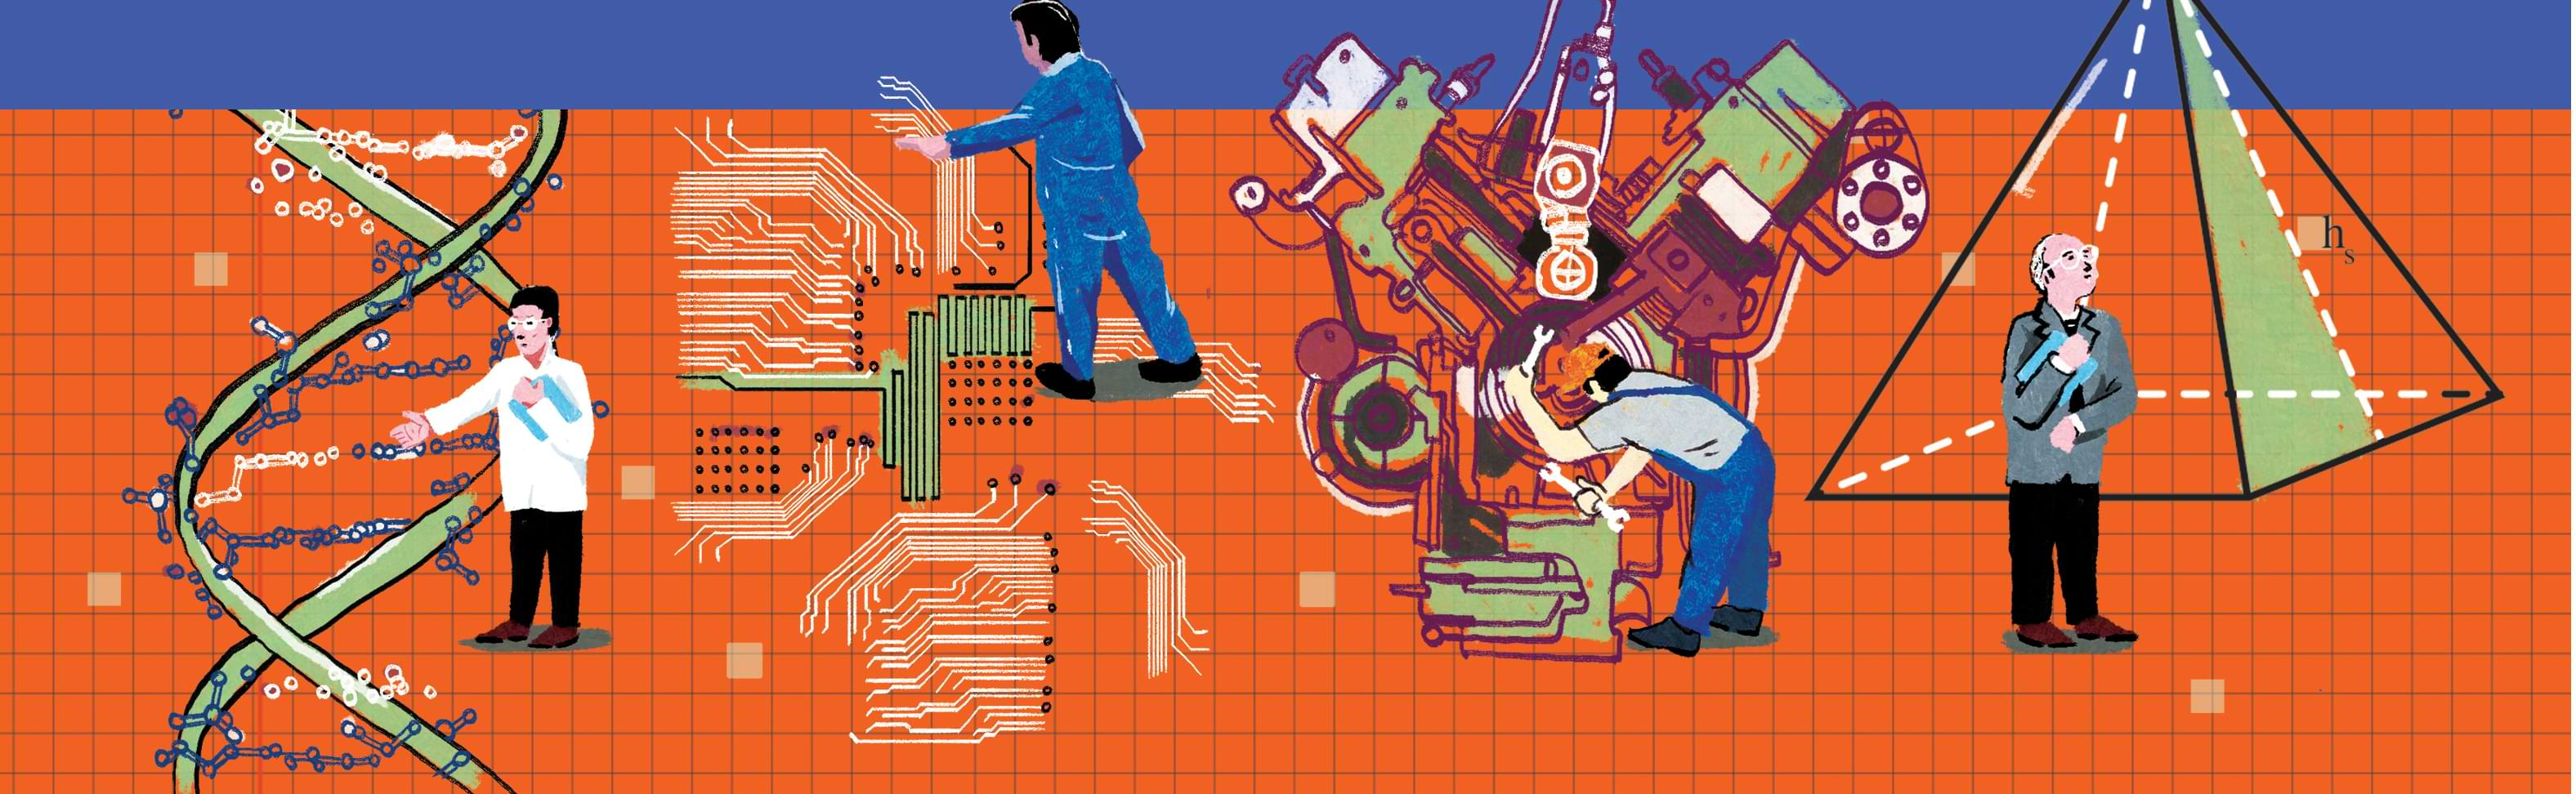
\includegraphics[width=19.3cm]{../bannertimhieu}}}
\AddToShipoutPicture*{\put(95,525){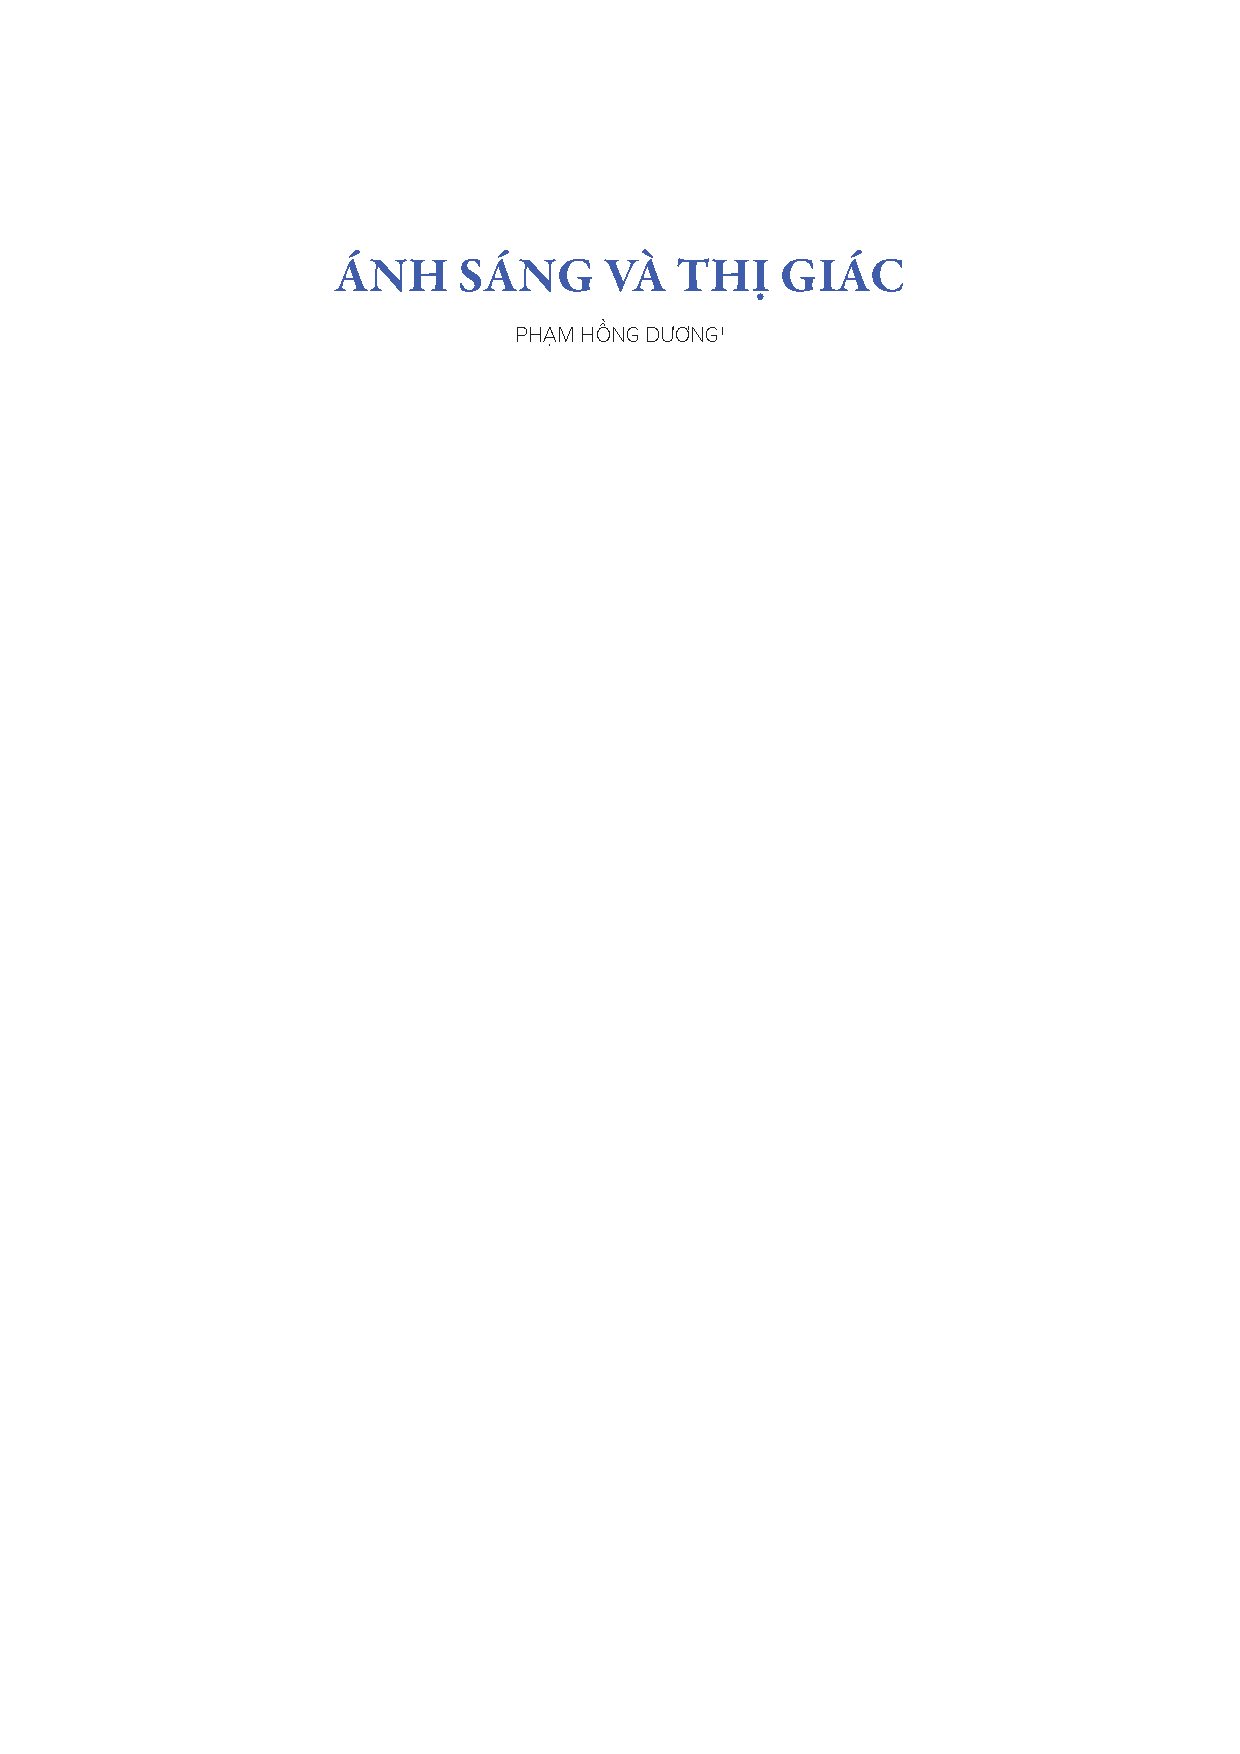
\includegraphics[scale=1]{../tieude.pdf}}}
\centering
\endgroup
\vspace*{180pt}

\begin{multicols}{2}
	\textit{Tích có hướng xuất hiện muộn trong chương trình toán phổ thông và được sử dụng chủ yếu trong các kỹ thuật tìm pháp tuyến của mặt phẳng. Trong bài này, Pi sẽ giới thiệu với các bạn về vai trò của tích có hướng trong vật lí liên quan đến lực Coriolis, một loại lực có ảnh hưởng đến nhiều hiện tượng tự nhiên.}
	\vskip 0.1cm
	$\pmb{1.}$ \textbf{Lực Coriolis là gì?}
	\vskip 0.1cm
	Khi giải các bài toán vật lí, ta thường chọn hệ quy chiếu gắn với mặt đất rồi áp dụng định\linebreak luật $2$ của Newton. Trong phần lớn các trường hợp, hệ quy chiếu này đáp ứng được nhu cầu bài toán. Tuy vậy, về mặt bản chất, hệ quy chiếu gắn với mặt đất không phải là một hệ quy chiếu quán tính (hệ quy chiếu mà một vật đang ở trạng thái nghỉ và không có lực nào tác dụng lên nó thì sẽ không giữ nguyên trạng thái nghỉ) do bản thân Trái đất cũng quay quanh trục của nó.
	\vskip 0.1cm
	Ta hãy xét một điểm cố định trên mặt đất. Chọn một hệ quy chiếu đứng yên, không quay cùng với Trái đất. Ta có thể coi đây là một hệ quy chiếu quán tính. 
	\vskip 0.1cm
	Kí hiệu $\overrightarrow{\Omega}$ là vector biểu diễn vận tốc góc của chuyển động quay quanh trục của bản thân Trái đất. Do một ngày có $86400$ giây, vận tốc này có độ lớn $\dfrac{\2\pi}{86400}$ ($\dfrac{rad}{s}$). Phương của vector $\overrightarrow{\Omega}$ được chọn hướng về phía cực bắc.
		\begin{figure}[H]
		\vspace*{-10pt}
		\centering
		\captionsetup{labelformat= empty, justification=centering}
		
\includegraphics[width= 0.4\textwidth]{11}
		\caption{\small\textit{\color{timhieukhoahoc}Hình $1$. Hệ quy chiếu quán tính (không quay) và hệ quy chiếu quay (gắn với mặt đất).}}
		\vspace*{-10pt}
	\end{figure}
	Mỗi một điểm $M$ trên Trái đất có thể được xác định bằng một vector $\overrightarrow{r}$ trong hệ trục tọa độ gắn với hệ quy chiếu quán tính của ta. Khi Trái đất quay, vận tốc của điểm này có phương tiếp tuyến với bề mặt Trái đất, khoảng cách đến trục quay là $r\sin\alpha$ (Hình $2$). Độ lớn của vận tốc này bằng với tích của vận tốc góc và bán kính quay, tức là $\Omega r \sin\alpha$. Do đó, ta có thể sử dụng tích vô hướng và viết:
	\begin{align*}
		\left(\!\!\frac{d\overrightarrow{r}}{dt}\!\!\right) = \overrightarrow{\Omega} \times \overrightarrow{r}. \tag{$1$}
	\end{align*}
	\begin{figure}[H]
		\vspace*{-5pt}
		\centering
		\captionsetup{labelformat= empty, justification=centering}
		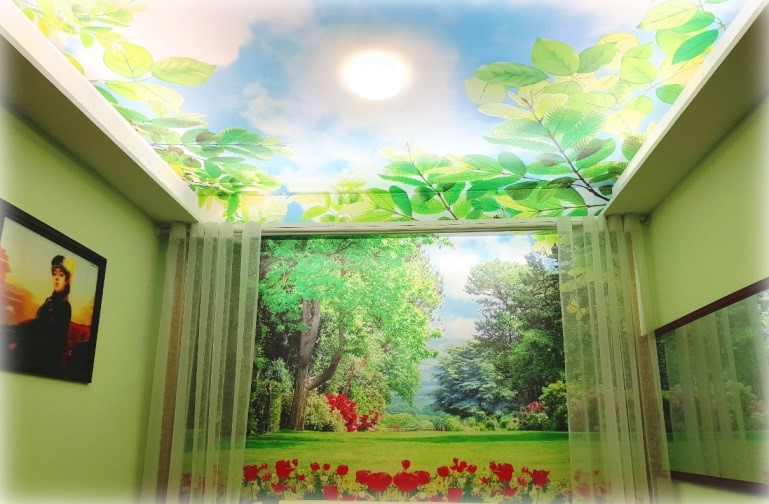
\includegraphics[width= 0.475\textwidth]{12}
		\caption{\small\textit{\color{timhieukhoahoc}Hình $2$. Ta có thể biểu diễn vận tốc của chuyển động quay bằng một tích có hướng.}}
		\vspace*{-10pt}
	\end{figure}
	\begin{tBox}
		\textit{Chú ý}: Ở đây, ta có một dạng kí hiệu mới là đạo hàm của vector theo thời gian. Trong khoảng thời gian rất nhỏ $\Delta t$, nếu một \linebreak vector từ $\overrightarrow{r_1}$ trở thành $\overrightarrow{r_2}$ thì ta có $\Delta\overrightarrow{r} = \overrightarrow{r_2}- \overrightarrow{r_1}$. Giới hạn của $\dfrac{\Delta\overrightarrow{r}}{\Delta t}$ khi $\Delta t$ tiến đến $0$ chính là đạo hàm của vector.
	\end{tBox}
	\vskip 0.1cm
	Ta cũng có thể mở rộng cho trường hợp điểm $P$ chuyển động so với mặt đất. Ta có:
	\begin{align*}
		\left(\!\!\frac{d\overrightarrow{r_P}}{dt}\!\!\right)\!\!_\textit{quán tính} \!=\! \left(\!\! \frac{d\overrightarrow{r_P}}{dt}\!\!\right)\!\!_{quay} \!+\! \overrightarrow{\Omega} \!\times\! \overrightarrow{r_P}. \tag{$2$}
	\end{align*}
	Ở đây, vận tốc của chất điểm trong hệ quy chiếu quán tính bằng với tổng vector của vận tốc của chất điểm trong hệ quy chiếu quay và vận tốc dài của chất điểm do chuyển động quay. Đây chính là tính tương đối của chuyển động.
	\vskip 0.1cm
	Không mất tính tổng quát, với một vector $\overrightarrow{u}$ bất kì, do vector được xác định bởi điểm đầu và điểm cuối, ta cũng có:
	\begin{align*}
		\left(\!\!\frac{d\overrightarrow{u}}{dt}\!\!\right)\!\!_\textit{quán tính} \!=\! \left(\!\!\frac{d\overrightarrow{u}}{dt}\!\!\right)\!\!_{quay} \!+\! \overrightarrow{\Omega} \!\times\! \overrightarrow{u}. \tag{$3$}
	\end{align*}
	Trở lại với điểm $P$, ta có thể viết ($2$) dưới dạng:
	\begin{align*}
		\overrightarrow{v}\!\!_\textit{quán tính} = \overrightarrow{v}\!\!_{quay} + \overrightarrow{\Omega} \times \overrightarrow{r_P}.
	\end{align*}
	Lấy đạo hàm, ta được (chú ý rằng $\overrightarrow{\Omega}$ là một vector bất biến):
	\begin{align*}
		&\left(\!\!\frac{d\overrightarrow{v}\!\!_\textit{quán tính}}{dt}\!\!\right)\!\!_\textit{quán tính} \\
		= &\left(\!\!\frac{d\overrightarrow{v}\!\!_{quay}}{dt}\!\!\right)\!\!_\textit{quán tính} + \overrightarrow{\Omega} \times \left(\!\!\frac{d\overrightarrow{r_P}}{dt}\!\!\right)\!\!_\textit{quán tính}
	\end{align*}
	Áp dụng ($3$) cho phương trình trên:
	\begin{align*}
		&\left(\!\!\frac{d\overrightarrow{v}\!\!_\textit{quán tính}}{dt}\!\!\right)\!\!_\textit{quán tính} = \left(\!\!\frac{d\overrightarrow{v}\!\!_{quay}}{dt}\!\!\right)\!\!_{quay} \\
		&+ \overrightarrow{\Omega}\times \overrightarrow{v}\!\!_{quay} + \overrightarrow{\Omega}\times\left(\!\!\overrightarrow{v}\!\!_{quay} + \overrightarrow{\Omega}\times\overrightarrow{r_p}\!\!\right).
	\end{align*}
	Đặt $\overrightarrow{a}\!\!_\textit{quán tính} = \left(\!\!\frac{d\overrightarrow{v}\!\!_\textit{quán tính}}{dt}\!\!\right)\!\!_\textit{quán tính}$ và $\overrightarrow{a}\!\!_{quay} = \left(\!\!\frac{d\overrightarrow{v}\!\!_{quay}}{dt}\!\!\right)\!\!_{quay}$ là gia tốc của chất điểm $P$ trong hệ quy chiếu quán tính và hệ quy chiếu quay, ta có:
	\begin{align*}
		&\overrightarrow{a}\!\!_\textit{quán tính} \\
		= &\overrightarrow{a}\!\!_{quay} + 2\overrightarrow{\Omega}\times \overrightarrow{v}\!\!_{quay} + \overrightarrow{\Omega}\times \left(\!\!\overrightarrow{\Omega} \times \overrightarrow{r_P}\!\!\right).
	\end{align*}
	Viết lại dưới dạng định luật $2$ của Newton:
	\begin{align*}
		m \overrightarrow{a}\!\!_{quay} =& m \overrightarrow{a}\!\!_\textit{quán tính} - 2m\overrightarrow{\Omega}\times \overrightarrow{v}\!\!_{quay}\\
		&- m \overrightarrow{\Omega}\times\left(\!\!\overrightarrow{\Omega} \times \overrightarrow{r_P}\!\!\right).
	\end{align*}
	Có thể thấy, khi ta chuyển từ hệ quy chiếu quán tính sang hệ quy chiếu quay thì sẽ xuất hiện thêm hai thành phần mới có vai trò lực quán tính. Thành phần $-\overrightarrow{\Omega}\times\left(\!\!\overrightarrow{\Omega}\times\overrightarrow{r_P}\!\!\right)$ chính là lực quán tính li tâm nằm trong mặt phẳng chứa trục quay, có phương vuông góc với trục quay và hướng ra xa trục quay. Còn thành phần $-2m\overrightarrow{\Omega}\times\overrightarrow{v}\!\!_{quay}$ được nhà toán học người Pháp, Gustave--Gaspard Coriolis, tìm ra và được đặt tên theo tên ông.
	\vskip 0.1cm
	Coriolis là một người đi tiên phong trong công cuộc cải tổ cách dạy và học môn cơ học. Các cuốn sách cơ học thời đó chỉ chú trọng về tĩnh học nên ứng dụng của chúng bị hạn chế trong ngành xây dựng. Trong các công trình của mình, Coriolis đã đưa ra các khái niệm về công, động năng, và định lý biến thiên động năng. Các cuốn sách của ông đã giúp đưa cơ học vào nhiều ngành nghề công nghiệp khác nhau. Những nghiên cứu về hệ qui chiếu quay ban đầu của ông không liên hệ đến chuyển động quay của Trái đất mà là về chuyển động quay các thiết bị như bánh xe nước.	
%	\vskip 0.1cm
		\begin{figure}[H]
		\vspace*{-5pt}
		\centering
		\captionsetup{labelformat= empty, justification=centering}
		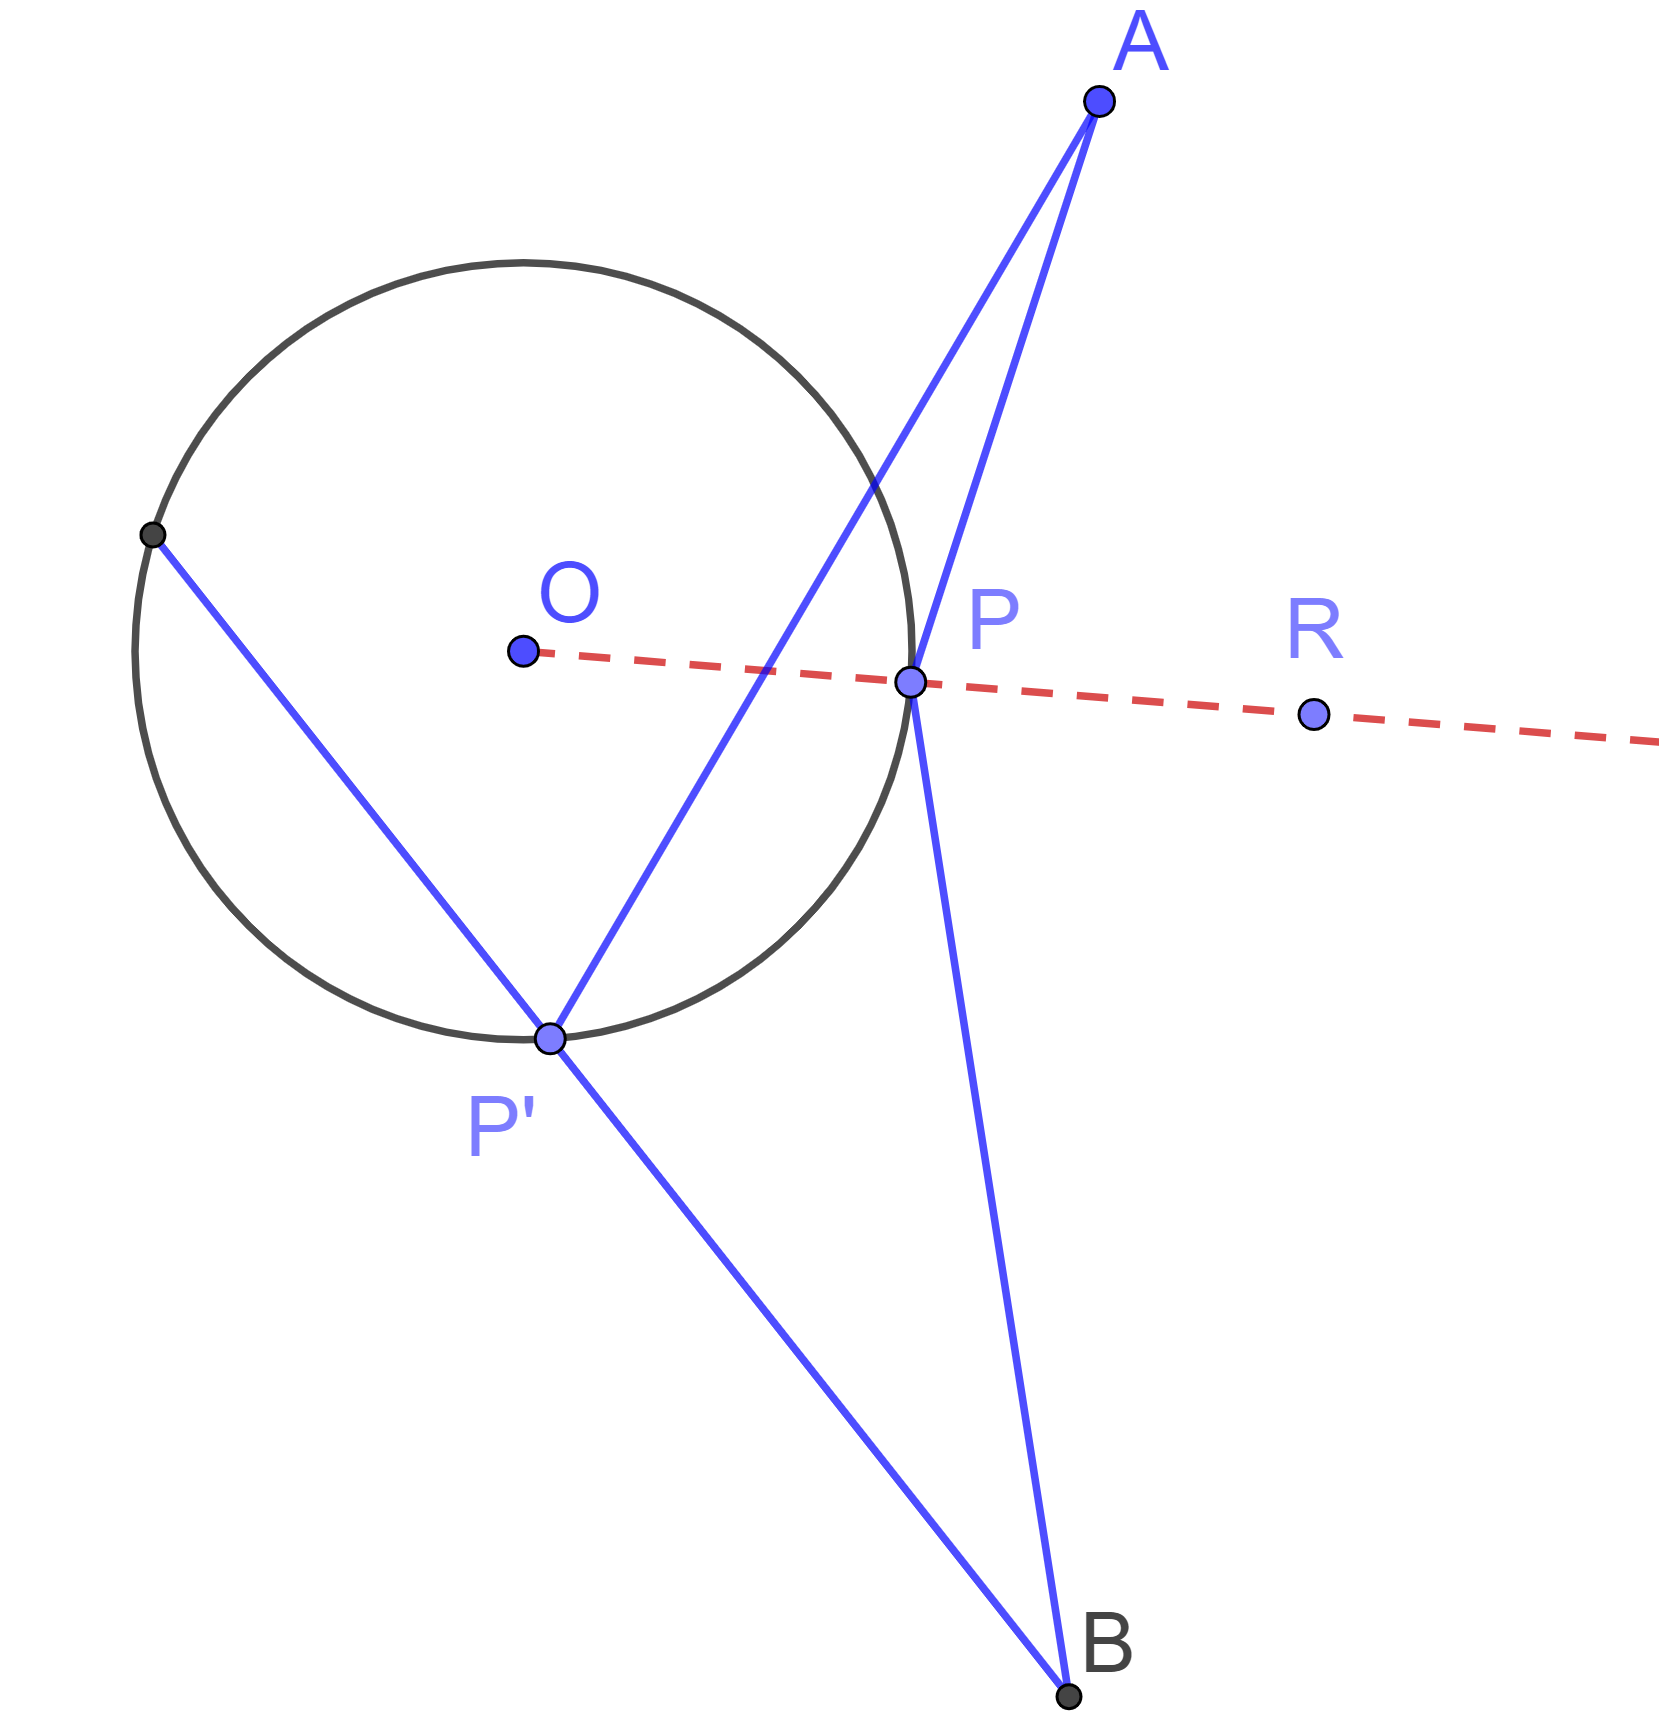
\includegraphics[width= 0.3\textwidth]{13}
		\caption{\small\textit{\color{timhieukhoahoc}Gustave--Gaspard Coriolis $(1812-1866)$}}
		\vspace*{-10pt}
	\end{figure}
	Năm $1851$, nhà khoa học người Pháp, Leon Foucault đã tiến hành một thí nghiệm chứng minh sự tồn tại của lực Coriolis. Ông sử dụng một con lắc đơn có dây treo dài $20$ m được gắn với trần nhà. Theo thời gian, người ta thấy mặt phẳng mà nó dao động trong đó sẽ thay đổi bằng cách so với các vạch được đánh dấu trên sàn nhà.
	\begin{figure}[H]
		\vspace*{-5pt}
		\centering
		\captionsetup{labelformat= empty, justification=centering}
		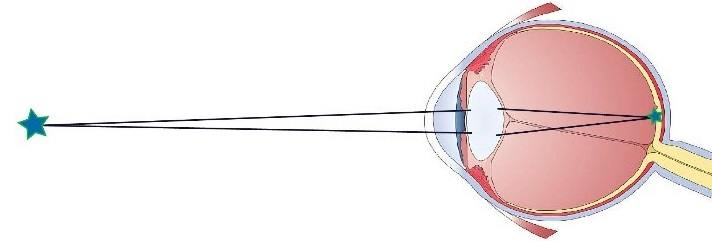
\includegraphics[height= 0.21\textwidth]{14}
		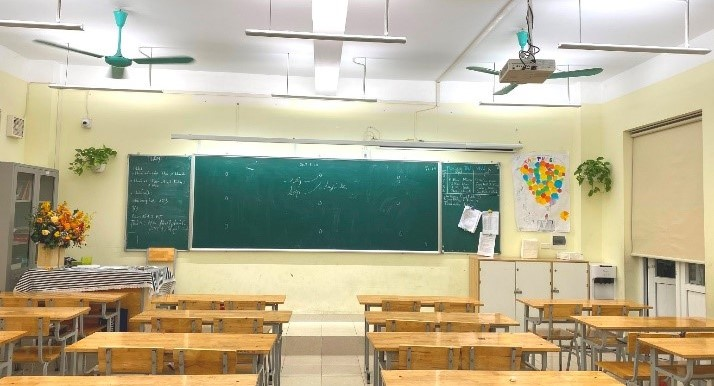
\includegraphics[height= 0.21\textwidth]{15}
		\caption{\small\textit{\color{timhieukhoahoc}Hình $3$. Con lắc Foucault có mặt phẳng dao động thay đổi theo thời gian.}}
		\vspace*{-10pt}
	\end{figure}
	Con lắc Foucault là một thí nghiệm rõ ràng nhất chứng minh sự tồn tại của lực Coriolis \linebreak do chuyển động quay quanh trục của Trái đất. Ta cũng cần chú ý rằng đây không phải là một lực thật giống như trọng lực mà là một dạng lực quán tính sinh ra do việc chuyển sang một hệ quy chiếu phi quán tính, tương tự như lực quán tính li tâm.
	\vskip 0.1cm
	$\pmb{2.}$ \textbf{Lực Coriolis ở hai bán cầu}
	\vskip 0.1cm
	Ta hãy xét trường hợp chất điểm có vận tốc theo phương Bắc -- Nam song song với mặt đất (vận tốc sẽ có phương tiếp tuyến với mặt cầu dọc theo kinh tuyến). Khi đó lực Coriolis\linebreak sẽ có phương vuông góc với chuyển động và cũng tiếp tuyến với mặt cầu. Ở Bán cầu Bắc, lực này sẽ luôn hướng sang phía phải của chuyển động còn ở Bán cầu Nam, lực sẽ luôn hướng sang phía trái của chuyển động. Độ lớn của lực sẽ là $2m\Omega v\sin\phi$ với $\phi$ là vĩ độ của chất điểm còn $v$ là vận tốc của chuyển động. Chú ý rằng tại xích đạo, nếu vận tốc có phương dọc theo kinh tuyến thì nó sẽ song song với trục quay và lực Coriolis bằng $0$.
	\begin{figure}[H]
		\vspace*{-5pt}
		\centering
		\captionsetup{labelformat= empty, justification=centering}
		
\includegraphics[width= 0.4\textwidth]{16}
		\caption{\small\textit{\color{timhieukhoahoc}Hình $4$. Khi vận tốc của vật (vector màu đỏ) có phương Bắc -- Nam, vector lực Coriolis (màu xanh) sẽ có phương Đông Tây, và chiều phụ thuộc vào chiều của vận tốc cùng bán cầu hiện tại. Góc giữa vector vận tốc và vector vận tốc góc cũng chính là vĩ độ.}}
		\vspace*{-10pt}
	\end{figure}
	Còn trong trường hợp chất điểm có vận tốc theo phương Đông -- Tây thì tình huống sẽ phức tạp hơn. Khi đó, lực Coriolis sẽ nằm trong mặt phẳng chứa trục quay và có phương vuông góc với trục quay. Ta có thể phân tích nó thành hai thành phần: một thành phần dọc theo phương bán kính từ tâm Trái đất và một thành phần tiếp tuyến với bề mặt Trái Đất. Thành phần tiếp tuyến này cũng luôn hướng về bên phải chuyển động ở Bán cầu Bắc và hướng về bên trái chuyển động ở Bán cầu Nam. Về mặt độ lớn, \linebreak thành phần tiếp tuyến này cũng có độ lớn là $2m\Omega v \sin\phi$.
%	\vskip 0.1cm
			\begin{figure}[H]
		\vspace*{-5pt}
		\centering
		\captionsetup{labelformat= empty, justification=centering}
		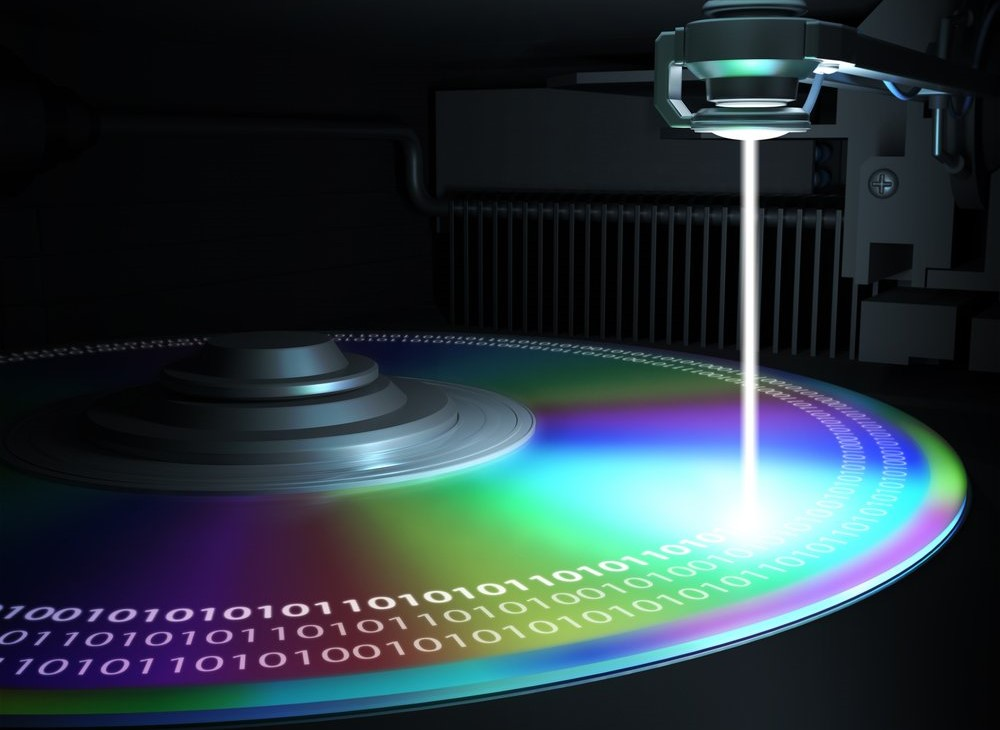
\includegraphics[width= 0.4\textwidth]{17}
		\caption{\small\textit{\color{timhieukhoahoc}Hình $5$. Trường hợp vật chuyển động từ Tây sang Đông. Lực Coriolis (màu xanh) sẽ nằm trong mặt phẳng chứa trục quay và vuông góc với trục quay. Trong trường hợp vật đi từ Đông sang Tây, lực Coriolis sẽ có chiều ngược lại.}}
		\vspace*{-10pt}
	\end{figure}
	Còn về thành phần dọc theo phương bán\linebreak kính Trái Đất, nó gây ra một hiệu ứng rất thú vị: hiệu ứng Eötvös, theo tên của nhà vật lí học người Hungary. Khi đi trên một tàu chở hàng của Đức, ông mang theo một thiết bị đo trọng lực nhận thấy rằng ở chiều đi về phía Đông thì trọng lực giảm còn ở chiều về phía Tây thì trọng lực lại tăng so với khi tàu đứng yên. Thật vậy, thành phần dọc theo phương bán kính Trái đất của lực Coriolis sẽ ngược chiều với trọng lực của vật khi đi về phía Đông và cùng chiều với trọng lực khi đi về phía Tây.
	\begin{figure}[H]
		\vspace*{-5pt}
		\centering
		\captionsetup{labelformat= empty, justification=centering}
		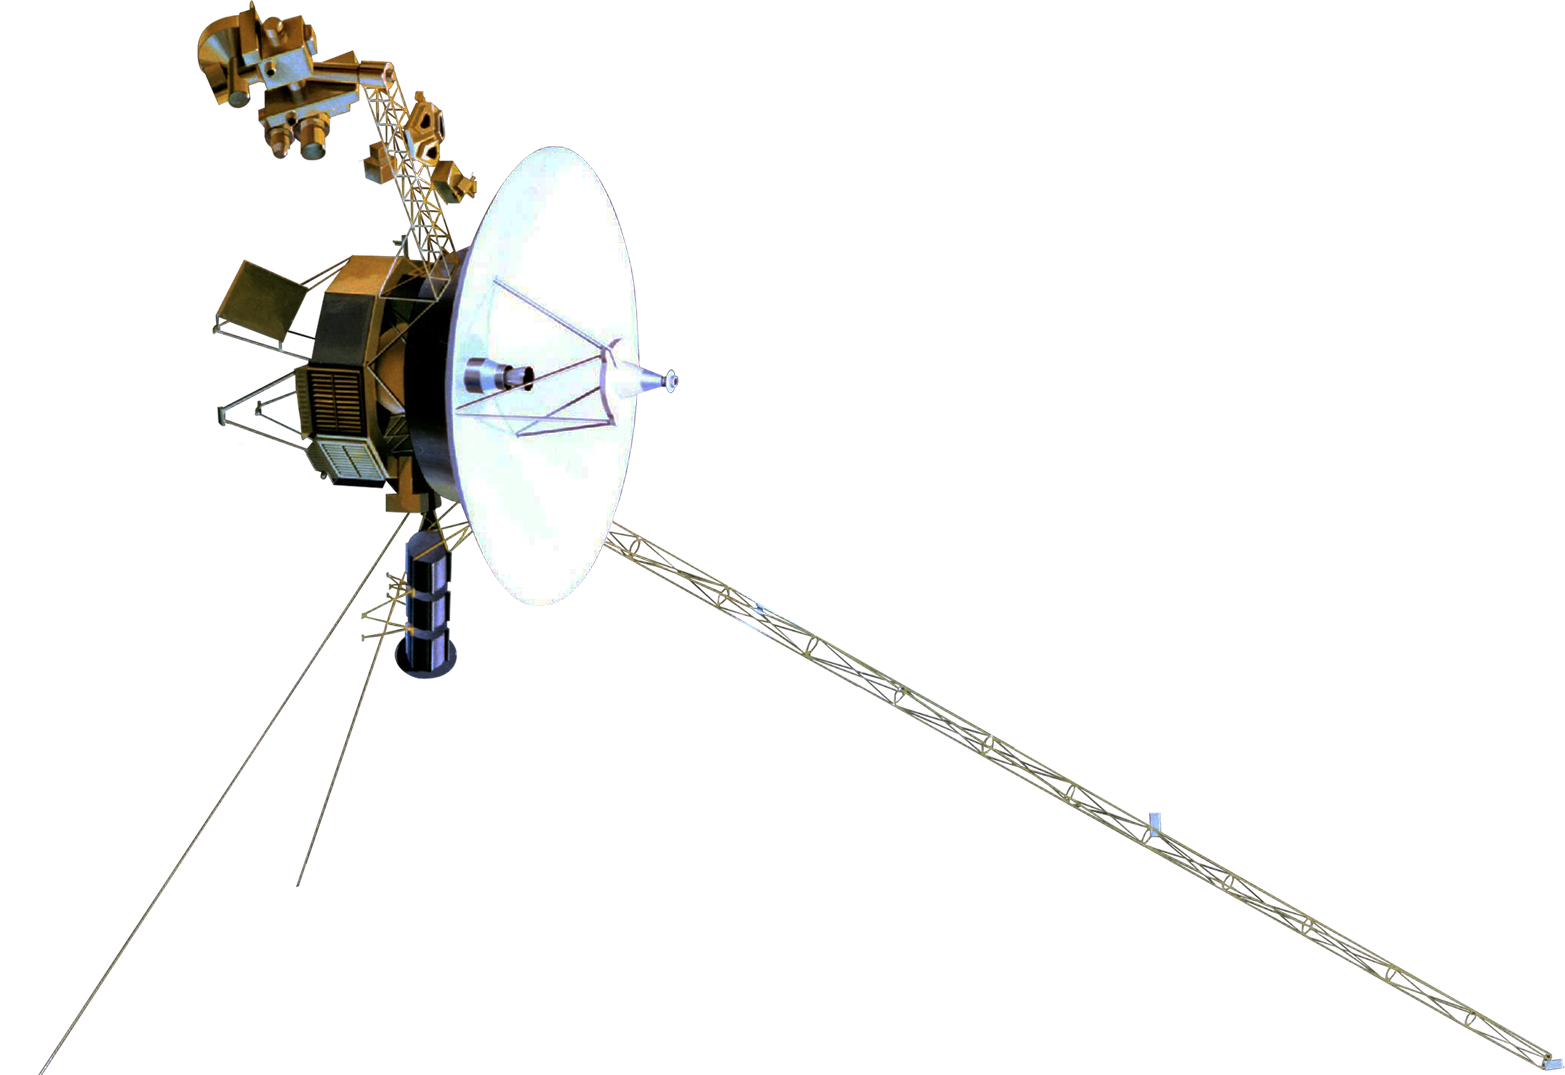
\includegraphics[width= 0.25\textwidth]{18}
		\caption{\small\textit{\color{timhieukhoahoc}Loránd Eötvös $(1848-1919)$}}
		\vspace*{-5pt}
	\end{figure}
	Khi vật có vận tốc song song với mặt đất, ta luôn có thể phân tích vận tốc của nó thành hai thành phần theo phương Bắc--Nam và Đông--Tây. Do đó, thành phần tiếp tuyến với mặt đất của lực Coriolis sẽ hướng về bên phải của chuyển động ở Bán cầu Bắc và hướng về bên trái chuyển động ở Bán cầu Nam với độ lớn $2m\Omega v\sin\phi$. Đây cũng là giải thích thường xuất hiện ở một số tài liệu về lực Coriolis khi không sử dụng tích có hướng. Tuy nhiên, cần chú ý rằng ở xích đạo ($\phi=0$), tuy thành phần song song với mặt đất của lực Coriolis bằng $0$, vẫn tồn tại thành phần theo phương thẳng đứng (tức phương bán kinh của Trái đất) khi vật chuyển động.
	\begin{figure}[H]
		\vspace*{-5pt}
		\centering
		\captionsetup{labelformat= empty, justification=centering}
		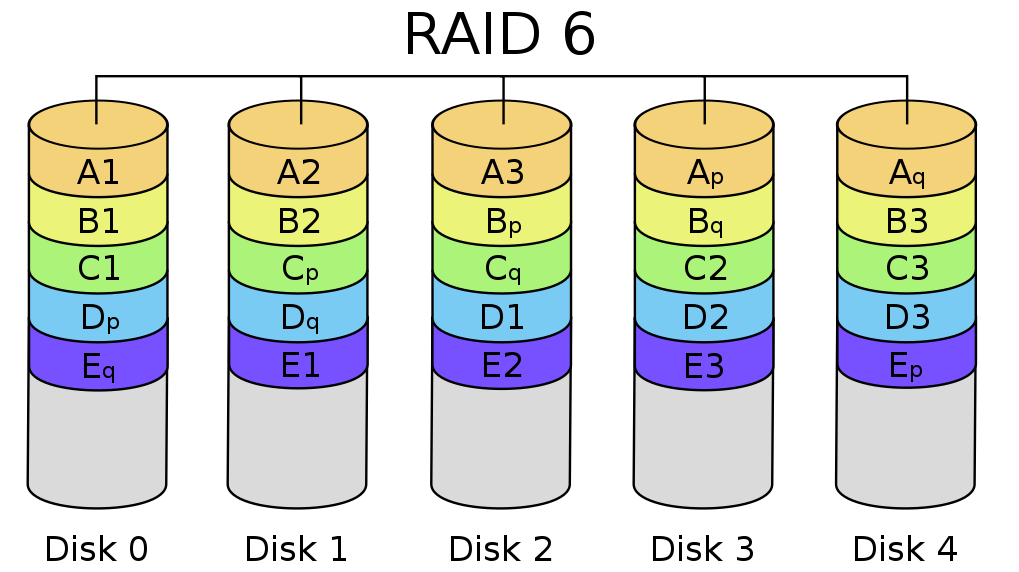
\includegraphics[width= 0.4\textwidth]{19}
		\caption{\small\textit{\color{timhieukhoahoc}Hình $6$. Chuyển động sẽ bị lệch về bên phải do lực Coriolis ở Bán cầu Bắc và về bên trái ở Bán cầu Nam. Ở vĩ độ càng cao, độ lệch sẽ càng lớn. Chuyển động ở xích đạo sẽ không bị lệch.}}
		\vspace*{-10pt}
	\end{figure}
	$\pmb{3.}$ \textbf{Lực Coriolis trong thực tiễn}
	\vskip 0.1cm
	Do Trái đất là hình cầu nên phía xích đạo nhận được nhiều ánh nắng hơn và có nhiệt độ cao hơn vùng cực. Nếu Trái đất không có chuyển động quay quanh trục, các luông gió chính sẽ chỉ thổi theo trục Bắc Nam ở mỗi bán cầu giữa vùng cực và xích đạo, tạo thành một vùng đối lưu duy nhất ở mỗi bán cầu.
	\vskip 0.1cm
	Do có lực Coriolis, chuyển động của không khí trong khí quyển không đơn giản như vậy. Các luồng gió chính sẽ bị lệch về bên phải ở Bán cầu Bắc và lệch về bên trái ở Bán cầu Nam. Hiện tượng này dẫn đến việc hình \linebreak thành ba chứ không phải một vùng đối lưu ở mỗi Bán cầu. Các vùng đối lưu này có ranh giới ở các vĩ độ $30$ độ và $60$ độ ở mỗi bán cầu bởi ở các vĩ độ này, lực Coriolis đã uốn các luồng gió thành gần như theo phương Đông -- Tây.
	\vskip 0.1cm 
	Chính bởi việc lực Coriolis làm các luồng gió chính bị lệch đi mà khí hậu trên Trái đất mới trở nên đa dạng và phức tạp như hiện nay. Đặc biệt, những luồng gió xiên ở gần xích đạo đã từ lâu được con người sử dụng để đi lại trên biển bằng thuyền buồm và được đặt tên là gió Mậu dịch (Trade wind). Nếu không có chúng, các con thuyền này chỉ có thể đi theo hướng Bắc Nam và sự giao thương giữa các nền văn minh Đông -- Tây trong lịch sử sẽ khó khăn hơn rất nhiều.
	\begin{figure}[H]
		\vspace*{-5pt}
		\centering
		\captionsetup{labelformat= empty, justification=centering}
		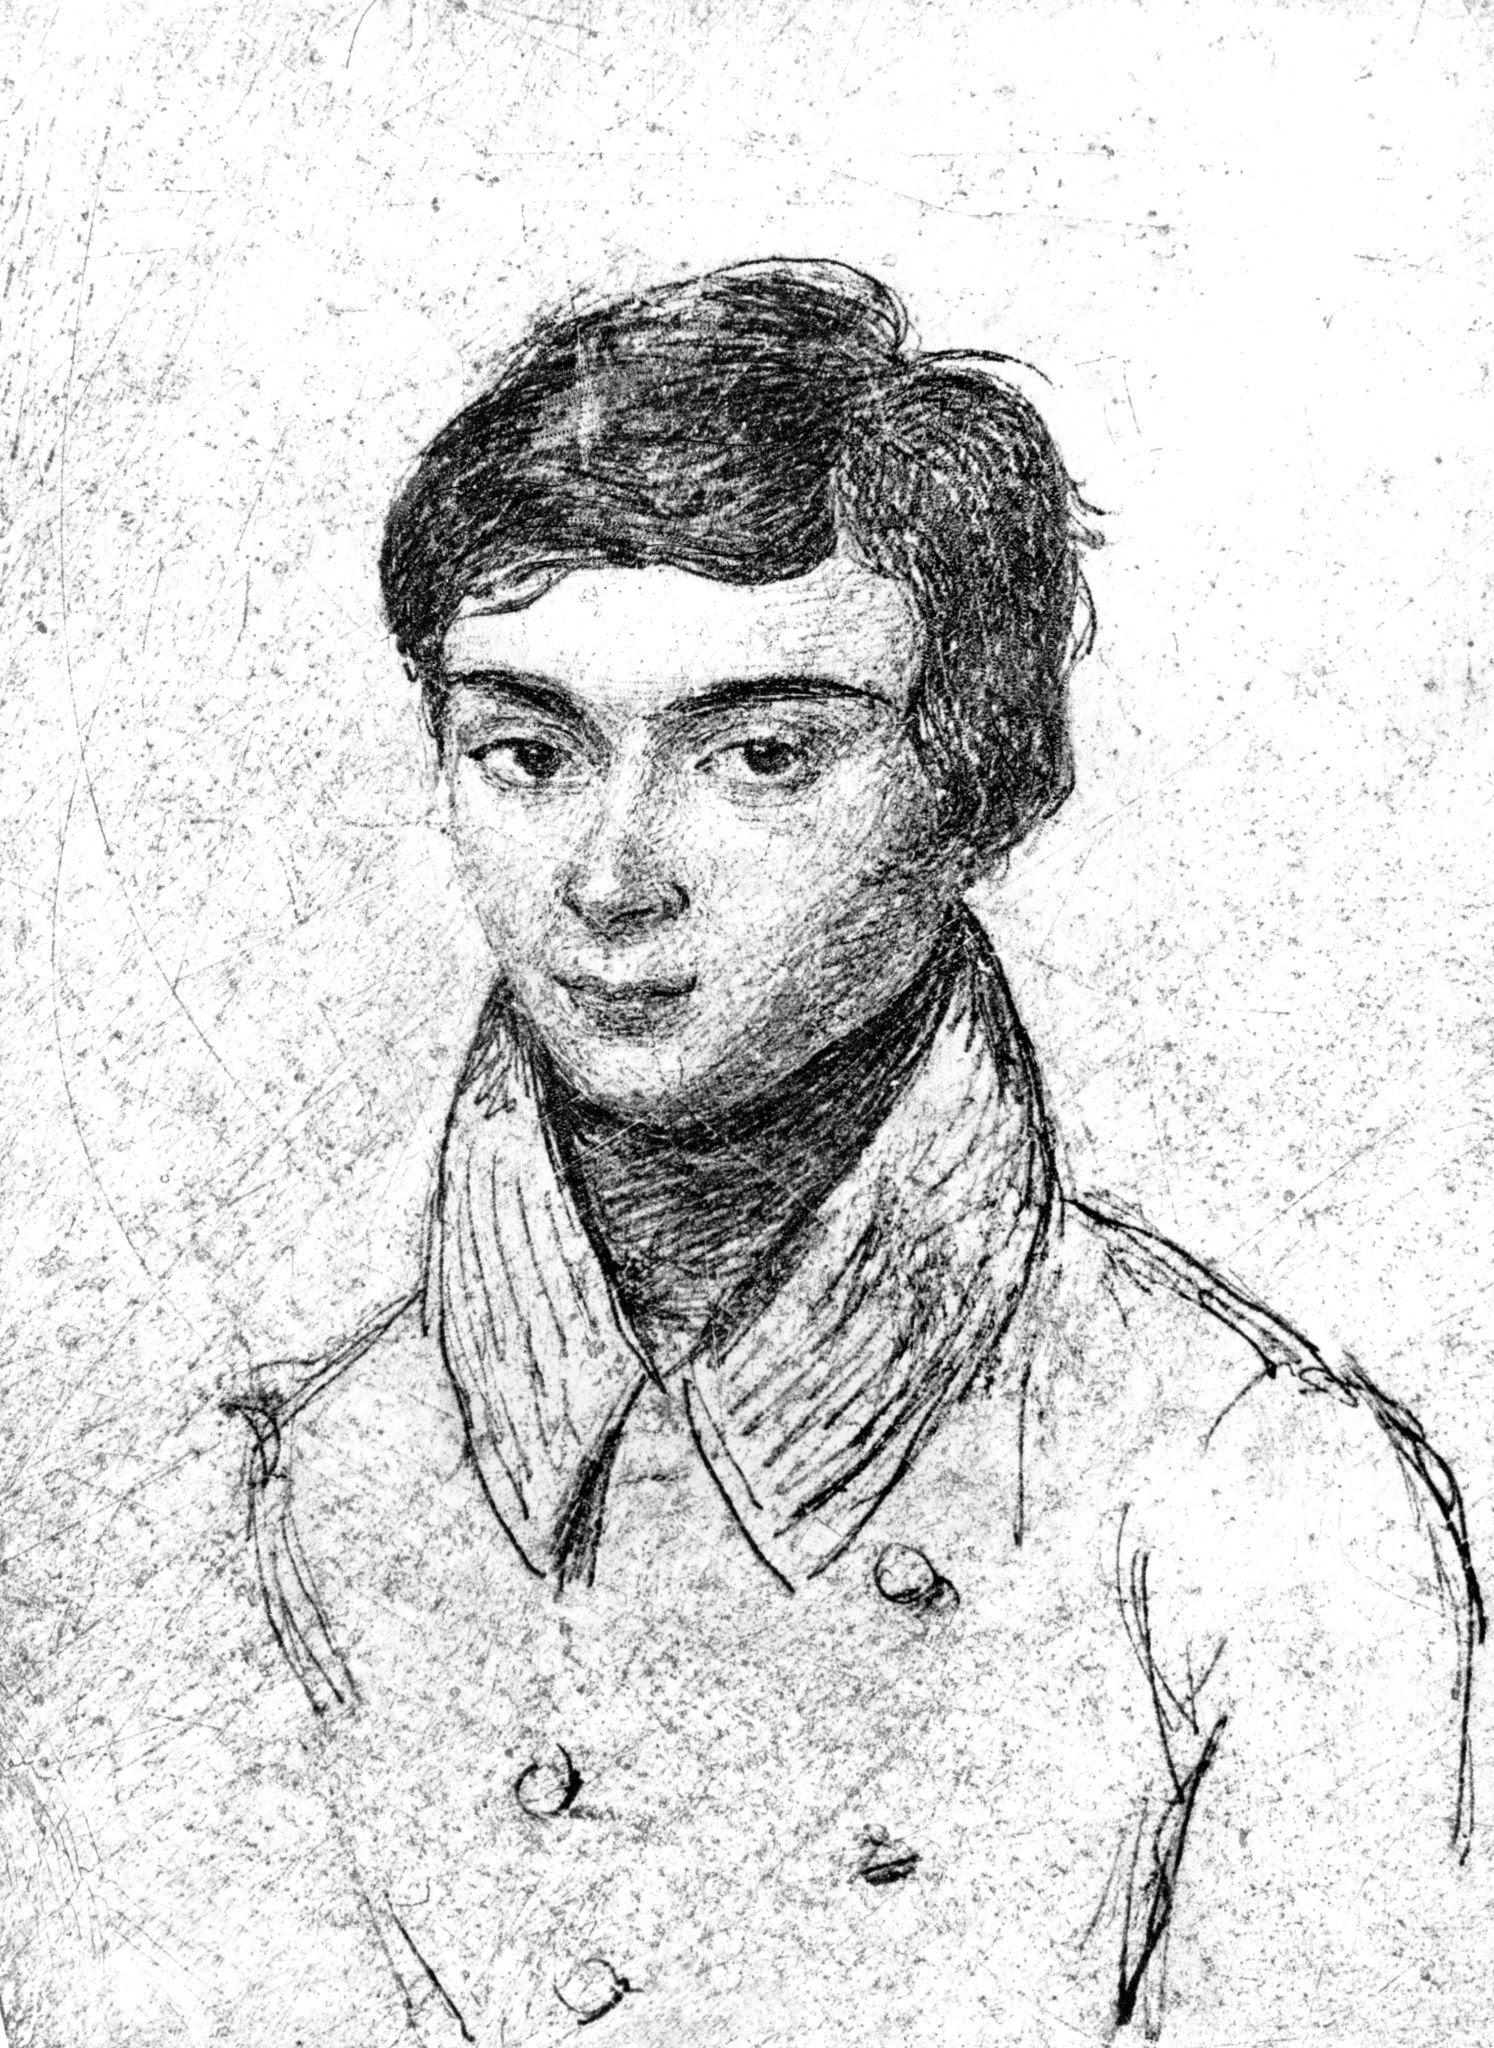
\includegraphics[width= 0.4\textwidth]{20}
		\caption{\small\textit{\color{timhieukhoahoc}Hình $7$. Các vùng đối lưu khác nhau của khí quyển Trái đất, được hình thành do lực Coriolis.}}
		\vspace*{-10pt}
	\end{figure}
	Lực Coriolis còn có một ảnh hưởng khác đến khí quyển: do nó luôn vuông góc với phương chuyển động nên các cơn bão hình thành ở hai bán cầu của Trái dất sẽ có chiều xoáy ngược nhau: ngược chiều kim đồng hồ ở Bán cầu Bắc và cùng chiều kim đồng hồ ở Bán cầu Nam. 
	\begin{figure}[H]
		\vspace*{-5pt}
		\centering
		\captionsetup{labelformat= empty, justification=centering}
		\includegraphics[height= 0.22\textwidth]{21}
		\includegraphics[height= 0.22\textwidth]{22}
		\caption{\small\textit{\color{timhieukhoahoc}Hình $8$. Các cơn bão ở Bán cầu Bắc (trái) có chiều xoáy ngược chiều kim đồng hồ còn các cơn bão ở Bán cầu Nam (phải) có chiều xoáy cùng chiều kim đồng hồ.}}
		\vspace*{-10pt}
	\end{figure}
	Ta cũng có thể quan sát được hiện tượng tương tự với những dòng hải lưu ở hai bán cầu. Ảnh hưởng của lực Coriolis đến những dòng hải lưu chính làm thay đổi khí hậu của nhiều vùng bờ biển cũng như phân bố oxy và dinh dưỡng của hệ sinh thái đại dương.
	\begin{figure}[H]
		\vspace*{-5pt}
		\centering
		\captionsetup{labelformat= empty, justification=centering}
		\includegraphics[width= 0.475\textwidth]{23}
		\caption{\small\textit{\color{timhieukhoahoc}Hình $9$. Các dòng hải lưu ở hai bán cầu dưới ảnh hưởng của lực Coriolis.}}
		\vspace*{-10pt}
	\end{figure}
		\begin{figure}[H]
		\vspace*{-5pt}
		\centering
		\captionsetup{labelformat= empty, justification=centering}
		\includegraphics[width= 0.4\textwidth]{24}
		\caption{\small\textit{\color{timhieukhoahoc}Hình $10$. Trên những hành tinh khác như sao Mộc, tốc độ quay quanh trục của hành tính lớn hơn nhiều so với Trái đất nên ta có thể quan sát rõ việc các luồng gió phương Bắc--Nam bị chuyển thành phương Đông--Tây do lực Coriolis cùng nhiều vành đai gió hình thành do hiện tượng này.}}
		\vspace*{-10pt}
	\end{figure}
	Không chỉ ảnh hướng đến khí quyển và đại dương, lực Coriolis còn là một chủ đề được quan tâm của ngành đạn đạo học. Ảnh hưởng của nó được chú ý đến nhiều từ năm $1918$, khi pháo binh Đức tiến hành pháo kích Paris từ khoảng các xa $120$ km với những đại bác cỡ lớn. Do khoảng thời gian bay của đạn dài hơn so với những loại súng nhỏ hơn trước đó, ảnh hưởng của lực Coriolis trở nên lớn hơn và đạn pháo bị lệch so với tính toán đến hơn $1$ km. Các kỹ sư pháo binh Đức đã phải tiến hành hiệu chỉnh lại theo độ lệch này. Những người lính bắn tỉa ở các khoảng cách xa (trên $1$ km) cũng phải tính thêm đến ảnh hưởng của lực Coriolis (bên cạnh các nhân tố khác như hướng gió, ...) đến quỹ đạo của đạn.
	\vskip 0.1cm
	$\pmb{4.}$ \textbf{Một số ngộ nhận}
	\vskip 0.1cm
	Một câu chuyện thường được lưu truyền về lực Coriolis là nó khiến cho dòng nước khi tháo bồn rửa trong nhà bếp hoặc nhà vệ sinh\linebreak xoay theo chiều khác nhau ở hai bán cầu giống như với các cơn bão. Tuy nhiên, nhận định này là không đúng. Trong thực tế, có rất nhiều nhân tố như hình dạng của bồn, tốc độ chảy của dòng nước, ... ảnh hưởng đến dòng chảy và những yếu tố này có ảnh hưởng lớn hơn rất nhiều lần so với lực Coriolis. Chỉ với những thí nghiệm được thiết kế đặc biệt, lượng nước được để yên tĩnh sau nhiều ngày, người ta mới có thể quan sát được dòng xoáy dưới ảnh hưởng của lực Coriolis gây ra khi tháo nước. Cũng cần nói thêm rằng, những câu chuyện khác như chiều xoắn móc bám của các dây leo hay chiều xoăn của tóc phụ thuộc vào bán cầu mà ta đang ở cũng là không đúng.
	\vskip 0.1cm
	Ngay cả những hiện tượng lớn hơn như chiều xoáy của các cơn lốc xoáy hay bờ bên nào của dòng sông bị lở cũng không trực tiếp phụ thuộc vào vị trí xảy ra ở bán cầu nào bởi ở những trường hợp này, có nhiều nhân tố khác có ảnh hưởng lớn hơn lực Coriolis rất nhiều. Lực Coriolis chỉ thể hiện rõ rệt ảnh hưởng của nó với những hiện tượng nhất định như đã nêu ở phần trước.
	\vskip 0.1cm
	Do công trình của Coriolis sử dụng nhiều phép tính vector, đặc biệt là tích có hướng mà không phải ai cũng tiếp cận được, đã có một số nỗ lực giải thích lực Coriolis một cách “đơn giản hóa”, dựa trên nhận định rằng các vĩ độ khác nhau có vận tốc dài khác nhau nên khi một chất điểm chuyển động từ vĩ độ này sang vĩ độ khác cũng giống như người ta ném một quả bóng từ một đoàn tàu đang chạy sang một đoàn tàu đang chay song song với vận tốc lớn hơn. Cách giải thích dạng này đã có từ thế kỷ $18$, được George Hadley\linebreak $(1685-1768)$ đưa ra và được Joseph \linebreak Betrand $(1822-1900)$ tiếp tục sử dụng. Tuy nhiên, những lập luận dạng này có nhiều giả định ngộ nhận như gia tốc trong quá trình chuyển động là không đổi, ... và cũng không giải thích được rằng chuyển động dọc theo phương Đông--Tây cũng chịu ảnh hưởng của lực Coriolis. Dù vậy, chúng vẫn xuất hiện lặp đi lặp lại trong nghiều tài liệu phổ biến khoa học. Đây là một trong những điều cần tránh khi giới thiệu về lực Coriolis trong dạy và học.
	\vskip 0.1cm
	$\pmb{5.}$ \textbf{Lời kết}
	\vskip 0.1cm
	Lực Coriolis và những hiện tượng có liên quan có ý nghĩa rất lớn trong nhiều hiện tượng thực tiễn cũng như trong các ngành khoa học.  Những hiện tượng tự nhiên mà nó chi phối (gió, bão, hải dương, ...) ảnh hưởng trực tiếp đến cuộc sống của mỗi con người chúng ta. Ngay cả bản thân Coriolis\linebreak khi còn sống cũng không ngờ được rằng những nghiên cứu cơ học của mình lại có ảnh hưởng lớn đến nhiều ngành khoa học như khí tượng học và hải dương học như vậy. Bạn đọc có thể tìm hiểu thêm về các chi tiết lịch sử cùng một số ứng dụng khác của lực Coriolis qua phần tài liệu tham khảo.
	\vskip 0.1cm
	\textbf{Tài liệu tham khảo}
	\vskip 0.1cm
	[$1$] A. O., Persson. $2005$. ``The Coriolis Effect:\linebreak Four centuries of conflict between common sense and mathematics." \textit{History of Meteorology}.
	\vskip 0.1cm 
	[$2$] K., Silver. $2011$. \textit{An Intuitive Approach to the Coriolis Effect}. Uppsala University.
	\vskip 0.1cm
	[$3$] S. T., Thornton, and Marion J. B. $2004$. \textit{Classical Dynamics of Particles and Systems}. Thomson Learning.
\end{multicols}